\documentclass[conference]{IEEEtran}
\IEEEoverridecommandlockouts

% ---------------------------------------------------------------
% Packages
% ---------------------------------------------------------------
\usepackage[utf8]{inputenc}
\usepackage[T1]{fontenc}
\DeclareFontShape{T1}{ptm}{m}{scit}{<->ssub*ptm/m/sc}{}
\usepackage[french]{babel}
\usepackage{cite}
\usepackage{amsmath,amssymb,amsfonts}
\usepackage{algorithmic}
\usepackage{graphicx}
\usepackage{textcomp}
\usepackage{xcolor}
\usepackage{booktabs}
\usepackage{hyperref}
\usepackage{multirow}
\usepackage{microtype}

% ---------------------------------------------------------------
% Titre et auteurs
% ---------------------------------------------------------------
\title{Exploration d'architectures neuronales profondes pour l'évaluation du risque ordinal}

\author{
  \IEEEauthorblockN{Noé Cochet}
  \IEEEauthorblockA{\textit{Dép. d'informatique et de génie logiciel}\\
  Université Laval, Québec, Canada\\
  noe-pierre.cochet.1@ulaval.ca}
  \and
  \IEEEauthorblockN{Théo Fornier}
  \IEEEauthorblockA{\textit{Dép. d'informatique et de génie logiciel}\\
  Université Laval, Québec, Canada\\
  theo.fornier.1@ulaval.ca}
  \and
  \IEEEauthorblockN{Bilal Kefif}
  \IEEEauthorblockA{\textit{Dép. d'informatique et de génie logiciel}\\
  Université Laval, Québec, Canada\\
  bilal.kefif.1@ulaval.ca}
  \and
  \IEEEauthorblockN{Étienne Plante-Dubé}
  \IEEEauthorblockA{\textit{Dép. d'informatique et de génie logiciel}\\
  Université Laval, Québec, Canada\\
  etienne.plante-dube.1@ulaval.ca}
  \and
  \IEEEauthorblockN{Jean-Simon Ratté}
  \IEEEauthorblockA{\textit{Dép. d'informatique et de génie logiciel}\\
  Université Laval, Québec, Canada\\
  jean-simon.ratte.1@ulaval.ca}
  }

\begin{document}

\maketitle


\begin{abstract}
Ce travail explore l'application de méthodes d'apprentissage profond récentes au problème de
classification ordinale du risque en assurance-vie, en utilisant le jeu de données \textit{Prudential Life Insurance Assessment}. Ce jeu de données tabulaires, composé de 128~variables, présente un défi représentatif d'un domaine traditionnellement dominé par les méthodes de \textit{gradient boosting}. Nous comparons des modèles de référence fondés sur XGBoost et CatBoost à des architectures d'apprentissage profond récentes conçues pour les données tabulaires, notamment TabM et TabNet. Plusieurs variantes expérimentales sont étudiées~: utilisation de données non étiquetées par pseudo-étiquetage, régularisation (\textit{Dropout}, \textit{Batch Normalization}, \textit{Weight Decay}) et approche \textit{teacher--student} pour l'augmentation tabulaire synthétique. Une étude d'ablation permet d'isoler la contribution des composantes clés de l'architecture sélectionnée. Les résultats montrent que \textbf{CatBoost, en s'appuyant sur une stratégie inspirée des solutions gagnantes de la compétition, obtient les meilleures performances avec un QWK de~$0{,}6616$, confirmant la robustesse du \textit{gradient boosting} sur ce type de données tabulaires complexes.}
\end{abstract}

\begin{IEEEkeywords}
apprentissage profond, données tabulaires, classification ordinale, assurance-vie, semi-supervisé, transformer, gradient boosting
\end{IEEEkeywords}

\section{Introduction}

L'évaluation du risque lors de la souscription en assurance-vie repose traditionnellement sur de longs questionnaires médicaux destinés à déterminer l'éligibilité aux produits d'assurance. Depuis quelques années, les assureurs y ont intégré des algorithmes d'apprentissage automatique afin de réduire le recours aux examens médicaux complémentaires tout en limitant le risque additionnel de mortalité. Les données recueillies dans ces questionnaires comportent de nombreuses variables médicales, comportementales et démographiques. Le processus d'attribution d'une classe de risque à chaque client constitue ainsi un problème de classification ordinale à huit niveaux.

Sur ce type de données tabulaires structurées, les méthodes de \textit{gradient boosting} telles que XGBoost~\cite{chen2016xgboost}, LightGBM~\cite{ke2017lightgbm} et CatBoost~\cite{prokhorenkova2018catboost} demeurent l'état de l'art. Pourtant, l'essor récent d'architectures de réseaux de neurones profonds conçues spécifiquement pour les données tabulaires, comme les approches fondées sur l'attention et les modèles de fondation, laisse entrevoir un potentiel compétitif croissant pour l'apprentissage profond.

Ce projet, réalisé dans le cadre du cours GLO-7030, vise à évaluer dans quelle mesure les avancées récentes en apprentissage profond peuvent rivaliser avec les modèles de \textit{boosting} classiques sur un problème réel d'évaluation du risque de mortalité en assurance-vie. Notre objectif principal est de comparer des architectures modernes d'apprentissage profond dédiées aux données tabulaires (TabNet, TabM), au travers d'une étude d'ablation sur les composantes d'entraînement, et d'explorer des stratégies semi-supervisées ainsi que la génération de données synthétiques.

La suite de ce rapport est organisée comme suit~: la Section~\ref{sec:etat_art} présente l'état de l'art; la Section~\ref{sec:approche} décrit l'approche proposée; la Section~\ref{sec:methodo} détaille la méthodologie et les expérimentations; la Section~\ref{sec:resultats} présente et discute les résultats; la Section~\ref{sec:conclusion} conclut le rapport.

\section{État de l'art}
\label{sec:etat_art}

\subsection{Gradient Boosting pour les données tabulaires}

Les méthodes de \textit{gradient boosting} constituent depuis plusieurs années l'approche dominante pour les tâches d'apprentissage supervisé sur données tabulaires. XGBoost~\cite{chen2016xgboost} introduit un cadre d'optimisation scalable avec régularisation L1/L2 intégrée. LightGBM~\cite{ke2017lightgbm} améliore l'efficacité computationnelle grâce à une construction d'arbres feuille par feuille et un échantillonnage par gradient. CatBoost~\cite{prokhorenkova2018catboost} propose un traitement natif des variables catégorielles via un encodage ordonné.

\subsection{Apprentissage profond sur des données tabulaires}
\label{subsec:dl-tabulaire}

Plusieurs travaux récents ont tenté de combler l'écart de performance entre les réseaux de neurones et les méthodes de boosting sur les données tabulaires~\cite{grinsztajn2022tree}. Nous distinguons trois familles d'approches pertinentes pour notre étude.

\subsubsection{Architectures attentionnelles spécialisées}
TabNet~\cite{arik2021tabnet} est une architecture neuronale conçue spécifiquement pour les données tabulaires, fondée sur un encodeur séquentiel à étapes successives. À chaque étape de décision, un mécanisme d'attention \textit{sparsemax} sélectionne un sous-ensemble parcimonieux de variables (\emph{feature masking}), ce qui rend le modèle interprétable et limite le sur-ajustement en haute dimension. L'architecture combine une régularisation de parcimonie sur les masques à une perte supervisée standard, permettant un entraînement de bout en bout. Contrairement aux modèles de fondation, TabNet est entraîné directement sur le jeu de données cible.

\subsubsection{Approches d'ensemble paramétriquement efficaces}
TabM~\cite{gorishniy2024tabm} combine un MLP avec un mécanisme de \emph{BatchEnsemble} appliqué à chaque couche linéaire. Quelques adaptateurs légers transforment indépendamment le flux d'information, créant ainsi $k$ représentations parallèles tout en partageant les poids principaux. Cette architecture obtient la diversité d'un ensemble de $k$ modèles à un coût paramétrique quasi identique à un MLP seul. Les variantes TabM$^{\dagger}$ intègrent en entrée des \textit{embeddings} PiecewiseLinear qui discrétisent chaque variable continue avant projection dans un espace continu, améliorant la modélisation des non-linéarités.

\subsubsection{Modèles de fondation tabulaires (non retenus)}
TabPFN~\cite{hollmann2022tabpfn} est un modèle de fondation \emph{prior-fitted} entraîné sur des millions de jeux de données synthétiques bayésiens, permettant une inférence en contexte sans ré-entraînement. Dans notre cas, TabPFN n'a pas été retenu~: la version originale est limitée à des jeux de données de quelques milliers d'échantillons, alors que \textit{Prudential} en contient $59\,381$.

TabDPT~\cite{tabdpt2024} adapte l'architecture Transformer à l'apprentissage tabulaire via un pré-entraînement par \emph{deep pseudo-target}, exploitant des données non étiquetées pour améliorer les représentations apprises. TabDPT n'a pas été évalué dans le cadre de ce projet et constitue une piste d'amélioration discutée en Section~\ref{sec:ameliorations}.

\subsection{Classification ordinale}

La prédiction d'une variable cible catégorique ordonnée, telle que les niveaux de risque, nécessite des ajustements par rapport à la classification multi-classe standard pour préserver la hiérarchie entre les étiquettes. Une approche séminale consiste à transformer le problème en une série de tâches binaires cumulatives, permettant de modéliser la probabilité que la cible dépasse un seuil donné \cite{frank2001simple}.

Au-delà de la décomposition des classes, l'enjeu réside dans l'optimisation de fonctions de perte sensibles à l'ordre. La \textit{Earth Mover's Distance} (EMD), ou distance de Wasserstein, est particulièrement adaptée puisqu'elle pénalise les erreurs proportionnellement à la distance entre la classe prédite et la classe réelle \cite{hou2016squared}. Dans le contexte actuariel, cette approche est souvent complétée par l'optimisation directe ou indirecte du \textit{Quadratic Weighted Kappa} (QWK), qui mesure l'accord entre les évaluateurs en tenant compte de l'ampleur des désaccords.


\subsection{Apprentissage semi-supervisé et augmentation tabulaire}

L'apprentissage semi-supervisé offre des avenues prometteuses pour pallier la rareté des données étiquetées dans les domaines complexes. Pour les données tabulaires, cela se traduit souvent par le pseudo-étiquetage, où un modèle prédictif assigne des étiquettes provisoires aux données non étiquetées afin d'augmenter l'ensemble d'entraînement~\cite{lee2013pseudo}. Une autre méthode performante est le pré-entraînement auto-supervisé par auto-encodage, comme illustré par l'architecture VIME (\textit{Variational Information Maximizing Self-Supervised Learning})~\cite{yoon2020vime}, qui apprend des représentations robustes en reconstruisant des données corrompues.

Enfin, le paradigme \textit{teacher--student}, initialement conçu pour la distillation de connaissances, permet de transférer l'information apprise par un modèle complexe (le maître) vers un modèle plus léger ou entraîné sur des données synthétiques (l'élève)~\cite{hinton2015distilling}. Cette stratégie est particulièrement pertinente lors de l'utilisation de techniques d'augmentation tabulaire, où le modèle doit apprendre à généraliser à partir d'échantillons générés artificiellement pour équilibrer les classes minoritaires.


\section{Approche proposée}
\label{sec:approche}

\subsection{Vue d'ensemble}

Notre approche suit un cadre comparatif structuré en deux volets~: (1) l'établissement de lignes de base avec des modèles de \textit{gradient boosting}, et (2) l'exploration d'architectures d'apprentissage profond récentes adaptées aux données tabulaires, avec plusieurs variantes expérimentales.

\subsection{Description du jeu de données}

Le jeu de données \textit{Prudential Life Insurance Assessment}~\cite{kaggle_prudential} est composé de \textbf{$59\,381$} exemples d'entraînement et \textbf{$19\,765$} exemples de test, chacun décrit par 128~variables couvrant des caractéristiques médicales, comportementales et démographiques. La variable cible \texttt{Response} prend $8$~valeurs ordinales ($1$~à~$8$). La distribution des classes est \textbf{fortement déséquilibrée, avec une prédominance de la classe~$8$}.

Les variables peuvent être regroupées en~:
\begin{itemize}
  \item Variables continues (ex.~: \texttt{Ht}, \texttt{Wt}, \texttt{BMI})~;
  \item Variables catégorielles à haute cardinalité (ex.~: \texttt{Product\_Info\_2})~;
  \item Variables binaires de conditions médicales (ex.~: \texttt{Medical\_History\_*})~;
  \item Variables avec valeurs manquantes (ex.~: \texttt{Employment\_Info\_*}).
\end{itemize}

\subsection{Prétraitement}

Pour les modèles de \textit{gradient boosting}, l'imputation des valeurs manquantes des variables numériques continues a été réalisée par la médiane. Les variables catégorielles à haute cardinalité ont été transformées par \textit{target encoding} (encodage par la moyenne de la cible) afin de modéliser les relations complexes tout en limitant la dimensionnalité de l'espace des caractéristiques. Les variables présentant un taux de valeurs manquantes supérieur à un seuil critique (par ex. \texttt{Medical\_History\_10}) ont été exclues. Une étape d'ingénierie des caractéristiques (\textit{feature engineering}) a complété ce prétraitement~: des statistiques agrégées (moyenne et minimum) ont été extraites des variables binaires d'antécédents médicaux (\texttt{Medical\_Keyword\_*}) pour enrichir la représentation de l'historique clinique.

\subsection{Modèles de référence (\textit{Gradient Boosting})}

Les modèles de référence s'inspirent des solutions gagnantes issues de la compétition originale. Ces stratégies, initialement fondées sur XGBoost, ont été adaptées à des architectures de \textit{gradient boosting} contemporaines telles que CatBoost, ce qui permet de bénéficier d'une régularisation améliorée et d'un traitement optimisé des données tabulaires. Les modèles de référence suivants ont été entraînés, avec une optimisation systématique de leurs hyperparamètres~:
\begin{itemize}
  \item \textbf{XGBoost}~\cite{chen2016xgboost}~: \texttt{n\_estimators}~$=1200$, \texttt{learning\_rate}~$\approx 0{,}047$, \texttt{max\_depth}~$=5$, \texttt{min\_child\_weight}~$=200$~;
  \item \textbf{CatBoost}~\cite{prokhorenkova2018catboost}~: \texttt{n\_estimators}~$=2000$, \texttt{learning\_rate}~$\approx 0{,}0615$, \texttt{max\_depth}~$=6$, \texttt{l2\_leaf\_reg}~$=10{,}0$, \texttt{random\_strength}~$=2{,}0$.
\end{itemize}

\subsection{Architectures d'apprentissage profond}

\subsubsection{TabNet}
\textbf{[DÉCRIRE L'UTILISATION DE TABNET]} : configuration, adaptation au problème ordinal, limites de scalabilité rencontrées.

\subsubsection{TabM}
TabM~\cite{gorishniy2024tabm} repose sur un mécanisme de \textit{BatchEnsemble} appliqué à chaque couche linéaire d'un MLP standard. Pour chaque couche, de 1~à~3 adaptateurs légers (scalaires d'entrée $r_i$, de sortie $s_i$ et de biais $b_i$, avec $i \in \{1,\ldots,k\}$) transforment le flux d'information de façon indépendante, créant ainsi $k$ représentations parallèles tout en partageant les mêmes poids principaux. Cette architecture permet d'obtenir la diversité d'un ensemble de $k$ modèles tout en conservant un coût paramétrique quasi identique à un MLP seul.

La structure globale et les mécanismes de partage de paramètres des quatre variantes étudiées (\textit{plain, packed, mini} et \textit{tabm}) sont synthétisés à la Figure 1. Nous explorons quatre variantes issues de l'article~:
\begin{itemize}
  \item \textbf{plain} (MLP de base, sans ensemble)~;
  \item \textbf{tabm-packed} (ensemble de $k$ MLP indépendants, sans partage de poids)~;
  \item \textbf{tabm-mini} (adaptateur $R$ uniquement, un seul scalaire par membre)~;
  \item \textbf{tabm} (adaptateurs $R$, $S$ et $B$ combinés, variante complète).
\end{itemize}

Les variantes notées TabM$^{\dagger}$ dans l'article ajoutent en entrée des \textit{embeddings} PiecewiseLinear, qui discrétisent chaque variable continue en $B$ intervalles avant de la projeter dans un espace continu de dimension $d_e$, améliorant nettement la modélisation des non-linéarités.

\begin{figure}[htbp]
  \centering
  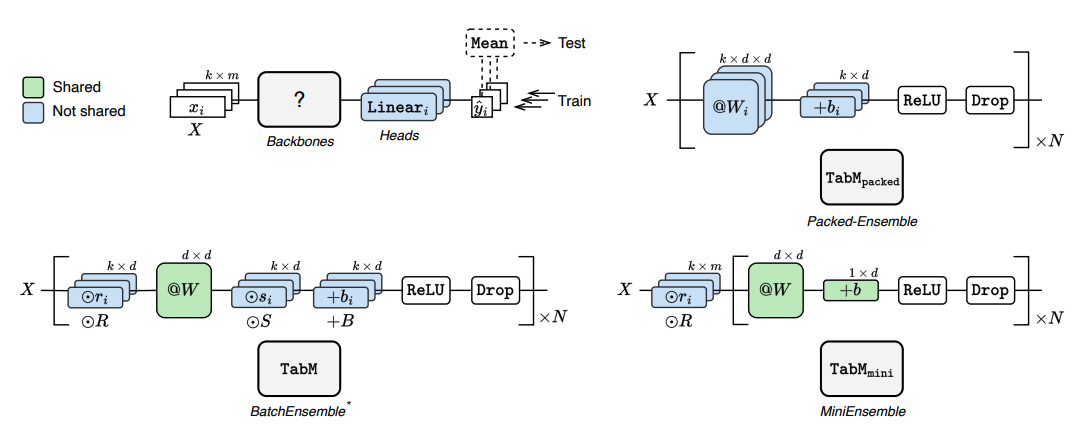
\includegraphics[width=\columnwidth]{Images/TabMarchi.png}
  \caption{Variantes d'architectures TabM~: schéma général (haut gauche),
  \textit{Packed-Ensemble} (haut droite), \textit{BatchEnsemble} utilisé
  dans TabM (bas gauche) et \textit{MiniEnsemble} (bas droite). En vert,
  les paramètres partagés entre les $k$ membres~; en bleu, les paramètres
  propres à chaque membre. Tiré de Gorishniy \textit{et al.}~\cite{gorishniy2024tabm}.}
  \label{fig:tabm_architectures}
\end{figure}

\subsection{Gestion de l'ordinalité}

\textbf{Décomposition binaire pour le \textit{boosting}~:} l'approche classique de régression a été substituée par une architecture de classification ordinale inspirée des meilleures solutions de la compétition, adaptée ici à XGBoost et à CatBoost. La classification ordinale est décomposée en sept classifieurs binaires prédisant successivement la probabilité de dépassement d'un seuil de classe ($y > 1$, $y > 2$, \ldots, $y > 7$). La somme de ces probabilités (augmentée de~1) fournit une prédiction continue. Plutôt que d'employer des seuils de discrétisation globaux, une calibration conditionnelle (\textit{variable split calibration}) est appliquée en partitionnant l'ensemble des prédictions selon la variable binaire \texttt{Medical\_History\_23}. Pour chaque sous-ensemble, les seuils sont initialisés à partir des percentiles de la distribution, puis optimisés par recherche locale (\textit{grid search}) afin de maximiser le QWK de validation. Couplée aux probabilités issues de CatBoost, cette optimisation des seuils apporte un gain absolu de QWK d'environ~$0{,}06$ par rapport à un arrondissement scalaire standard.

Pour adapter les modèles d'apprentissage profond à la nature ordinale de la cible ($8$~classes ordonnées, $y \in \{1, \ldots, 8\}$), nous adoptons une approche de \textbf{régression ordinale continue} plutôt qu'une classification multi-classes standard.

La tête de sortie des deux modèles produit un scalaire réel ($d_{\text{out}}=1$). La variable cible est standardisée avant l'entraînement~:
\begin{equation}
  \tilde{y} = \frac{y - \mu_y}{\sigma_y},
\end{equation}
où $\mu_y$ et $\sigma_y$ sont estimés sur l'ensemble d'entraînement. À l'inférence, la prédiction est dénormalisée puis arrondie à la classe ordinale la plus proche.

TabNet utilise la MSE comme fonction de perte. TabM, en revanche, optimise directement la métrique d'évaluation via une approximation différentiable du \textit{Quadratic Weighted Kappa} (QWK), la soft-QWK.

Le QWK est défini à partir d'une matrice de pondération quadratique qui pénalise les erreurs proportionnellement à leur écart ordinal~:
\begin{equation}
  W_{ij} = \frac{(i - j)^2}{(K-1)^2}, \quad i, j \in \{1, \ldots, K\}.
\end{equation}

La soft-QWK s'appuie sur une softmax pour relâcher la distribution et fait intervenir un hyperparamètre de température~$\tau$ qui contrôle la netteté de la distribution sur les classes~: un $\tau$~faible place presque tout le poids sur la classe la plus proche, tandis qu'un $\tau$~élevé l'étale sur les classes voisines.

Dans les deux cas, l'\textit{early stopping} est piloté par le QWK mesuré sur le jeu de validation à chaque époque.

\subsection{Utilisation de données synthétiques}

Dans le cadre de la prédiction du niveau de risque en assurance à partir de données tabulaires, nous avons été confrontés à plusieurs limitations classiques~: taille du jeu de données limitée, déséquilibre entre classes et difficulté à modéliser des relations complexes entre variables.

Les modèles d'apprentissage profond sont sensibles à la quantité de données disponibles~\cite{goodfellow2016deep}~: leur performance tend à augmenter avec le volume de données d'entraînement, contrairement à certains modèles tabulaires classiques (comme les méthodes de \textit{boosting}), souvent plus robustes en régime de faibles données.

Afin de pallier ces limitations, nous avons choisi d'explorer l'utilisation de données synthétiques pour enrichir le jeu de données initial. Notre approche repose sur un pipeline structuré en plusieurs étapes~:
\begin{enumerate}
    \item analyse du jeu de données initial (types de variables, distributions, corrélations)~;
    \item génération de données synthétiques conditionnées sur certaines classes~;
    \item évaluation de la cohérence des données générées~;
    \item augmentation du jeu de données réel~;
    \item entraînement et comparaison des modèles.
\end{enumerate}

Plusieurs modèles génératifs adaptés aux données tabulaires ont été étudiés.

\subsubsection{CTGAN}
Le modèle CTGAN~\cite{xu2019modeling} est une extension des GAN spécifiquement conçue pour les données tabulaires. Il permet de gérer les variables mixtes (numériques et catégorielles) via un mécanisme de conditionnement. Nous l'utilisons pour générer des données synthétiques conditionnées par classe, afin de mieux modéliser les distributions spécifiques à chacune.

\subsubsection{TVAE}
Le modèle TVAE (\textit{Tabular Variational Autoencoder})~\cite{xu2019modeling} repose sur une approche probabiliste permettant de modéliser la distribution jointe des variables. La même stratégie de génération conditionnée par classe est appliquée avec TVAE.

\subsubsection{TabSyn}
Nous avons également expérimenté TabSyn~\cite{zhang2024tabsyn}, une approche fondée sur des modèles de diffusion en espace latent pour la génération de données tabulaires. L'implémentation utilisée provient du dépôt officiel, que nous avons cloné et adapté à notre jeu de données. Cette approche permet elle aussi une génération conditionnée afin de capturer des distributions propres à chaque classe.

\subsubsection{Génération via LLM}
Nous avons également exploré l'utilisation de modèles de langage (LLM) comme générateurs conditionnels, à partir de \textit{prompts} structurés décrivant le format et les contraintes du jeu de données. Cette approche permet de produire des données synthétiques en contrôlant explicitement certaines caractéristiques via le \textit{prompt}, notamment la classe cible et la structure des variables.

Plusieurs modèles ont été testés, notamment GPT-5.3~Pro et Gemini~3.1~Pro. Parmi ceux-ci, GPT-5.3~Pro a produit les résultats les plus satisfaisants dans notre cadre expérimental.

\subsubsection{Diffusion pour données tabulaires}
Nous avons également étudié des approches fondées sur les modèles de diffusion, telles que TabDDPM~\cite{kotelnikov2023tabddpm}, qui reposent sur un processus de débruitage progressif pour générer les données. Toutefois, des contraintes liées aux dépendances logicielles et à la compatibilité de certaines bibliothèques ont limité leur intégration dans notre cadre expérimental.


\section{Méthodologie et expérimentation}
\label{sec:methodo}

\subsection{Protocole d'évaluation}

Tous les modèles sont évalués selon les métriques suivantes~:
\begin{itemize}
  \item \textbf{Kappa de Cohen quadratique pondéré (QWK)}~: métrique principale du concours Kaggle~;
  \item \textbf{Accuracy}~: taux de classification exacte~;
  \item \textbf{MAE ordinal}~: erreur absolue moyenne sur les niveaux de risque.
\end{itemize}

Nous utilisons une validation croisée stratifiée à $k=5$~plis pour tous les modèles supervisés. Les résultats sur l'ensemble de test Kaggle sont obtenus via soumission.

\subsection{Détails d'entraînement}

L'optimisation des hyperparamètres pour XGBoost et CatBoost a été réalisée par une recherche bayésienne (\textit{bayesian sweep}) de $100$~itérations orchestrée par \textit{Weights \& Biases} (W\&B). Les modèles ont été évalués sur une séparation stricte (\textit{split}~$80/20$) des données nettoyées, en utilisant le QWK de l'ensemble de validation comme critère d'arrêt précoce (\textit{early stopping}) après $50$~itérations sans amélioration. L'entraînement a été effectué sur le \textit{cluster} de calcul de l'Université Laval (n\oe uds ICE) avec accélération matérielle.

Pour les autres modèles, les paramètres généraux sont les suivants~:
\begin{itemize}
  \item Matériel utilisé (GPU/CPU, mémoire)~;
  \item Optimiseur (ex.~: Adam, AdamW), taux d'apprentissage, scheduler~;
  \item Nombre d'époques, \textit{early stopping}~;
  \item Taille de lot (\textit{batch size})~;
  \item Initialisation des poids.
\end{itemize}


\subsection{Méthodologie de génération des données synthétiques}

Pour chaque méthode de génération (CTGAN, TVAE, TabSyn), nous adoptons une spécialisation par classe~: le jeu d'entraînement est séparé selon la variable cible et un modèle distinct est entraîné pour chacune des huit classes. Cette approche permet de générer des données conditionnées de façon explicite, en sélectionnant directement la classe cible via le modèle utilisé lors de la génération.

\subsubsection{Stratégies de génération}
Plusieurs stratégies ont été mises en place afin d'évaluer l'impact de l'ajout de données synthétiques.

\paragraph{Stratégie A~: génération ciblée}
La stratégie~A consiste à ne générer des données que pour les classes sous-représentées. Le nombre d'exemples à produire est déterminé à partir de la distribution initiale~: les classes minoritaires sont augmentées jusqu'à atteindre $50\,\%$ de la taille de la classe majoritaire. Cette stratégie vise à réduire le déséquilibre sans modifier fortement la distribution globale.

Pour chaque classe sélectionnée, le modèle correspondant est chargé, puis un nombre spécifique d'échantillons est généré. Les données synthétiques produites sont ensuite~:
\begin{itemize}
    \item associées explicitement à leur classe cible~;
    \item dotées de nouveaux identifiants afin d'éviter tout conflit avec les données réelles~;
    \item réorganisées pour correspondre exactement à la structure du jeu de données original.
\end{itemize}
Les données générées pour chaque classe sont sauvegardées séparément, concaténées pour former un jeu de données synthétique global, puis fusionnées avec les données réelles afin de produire un jeu de données augmenté.

\paragraph{Stratégie B~: équilibrage complet}
La stratégie~B vise à générer des données synthétiques pour toutes les classes afin d'obtenir un jeu de données équilibré. Le nombre d'exemples générés est calculé de manière à atteindre un effectif similaire entre classes. Le processus de génération est identique à celui de la stratégie~A~:
\begin{itemize}
    \item chargement du modèle associé à chaque classe~;
    \item génération du nombre requis d'échantillons~;
    \item attribution de nouveaux identifiants~;
    \item alignement de la structure avec le jeu de données réel.
\end{itemize}
Les données synthétiques sont ensuite concaténées et fusionnées avec le jeu initial pour produire une version entièrement équilibrée.

\paragraph{Stratégie C~: classes 1 et 2}
La stratégie~C cible les classes pour lesquelles le modèle d'apprentissage profond présente le plus d'erreurs de prédiction, soit les classes~1 et~2. L'objectif est d'améliorer la performance du modèle sur ces classes en générant $20\,000$~exemples supplémentaires à l'aide des modèles correspondants. Comme pour les autres stratégies, les données synthétiques sont associées à leur classe cible, dotées de nouveaux identifiants et alignées avec la structure du jeu de données réel avant d'être fusionnées avec les données d'origine.

\paragraph{Stratégie D~: classes 4, 6 et 7}
La stratégie~D repose sur le même principe en ciblant les classes~4, 6 et~7, identifiées comme présentant un intérêt particulier pour la performance du modèle. Le processus de génération et d'intégration est identique à celui des autres stratégies~: génération conditionnée par classe, attribution de nouveaux identifiants et fusion avec le jeu de données réel.


\subsection{Variantes expérimentales}

\subsubsection{Expérience~1~: comparaison des modèles de base}
Comparaison directe de tous les modèles dans leur configuration standard sur les données d'entraînement avec prétraitement minimal.

\subsubsection{Expérience~2~: régularisation}
Évaluation de l'impact de différentes techniques de régularisation sur le modèle d'apprentissage profond retenu~: \textit{Dropout} ($p \in \{0{,}1\,;\, 0{,}3\,;\, 0{,}5\}$), \textit{Batch Normalization} et \textit{Weight Decay} ($\lambda \in \{10^{-4}, 10^{-3}, 10^{-2}\}$).

\subsubsection{Expérience~3~: utilisation des données non étiquetées}
Exploitation des données de test (sans étiquettes) via pseudo-étiquetage et/ou pré-entraînement par auto-encodage pour améliorer les représentations apprises.

\subsubsection{Expérience~4~: approche \textit{teacher--student} avec augmentation synthétique}
Un modèle enseignant (\textit{teacher}) entraîné sur les données réelles génère des pseudo-étiquettes sur un grand volume de données synthétiques. Le modèle élève (\textit{student}) est pré-entraîné sur ces données augmentées, puis affiné (\textit{fine-tuning}) sur les données originales.

\subsubsection{Expérience~5~: étude d'ablation TabM}
Nous isolons la contribution de chaque composante de TabM sur le jeu de données \textit{Prudential}. Six variantes sont entraînées dans des conditions identiques~: même optimiseur AdamW, \textit{scheduler} CosineAnnealingLR, \textit{early stopping} de patience~$10$, $k=32$~membres, 3~blocs de dimension~$512$ (2~blocs pour les variantes avec \textit{embeddings}, conformément à l'article). Un \textit{sweep} bayésien via Weights \& Biases explore ensuite l'espace des hyperparamètres de la meilleure variante (30~configurations, optimisation du QWK). Enfin, un \textit{stacking} combinant TabM$^{\dagger}$, XGBoost et LightGBM est évalué en validation croisée à $5$~plis.

\section{Résultats et Discussion}
\label{sec:resultats}

\subsection{Comparaison globale des modèles}

\begin{table}[htbp]
\caption{Comparaison des performances des modèles. La colonne « brut » donne le
QWK obtenu directement à partir des prédictions arrondies~; la colonne « +off » applique l'optimisation par
\textit{grid search} (et la \textit{Variable Split Calibration} pour les
modèles de \textit{boosting})~; la colonne « test Kaggle » correspond au score
privé sur l'ensemble de test caché.}
\label{tab:resultats_globaux}
\centering
\begin{tabular}{lccc}
\toprule
\textbf{Modèle} & \textbf{QWK\textsubscript{brut}} & \textbf{QWK\textsubscript{+off.}} & \textbf{QWK\textsubscript{Kaggle.}}\\
\midrule
XGBoost                  & --                  & $0{,}594$          & -- \\
CatBoost                 & --                  & $\mathbf{0{,}662}$ & $\mathbf{0{,}675}$ \\
MLP                      & $0{,}594$           & $0{,}632$          & -- \\
TabNet                   & --                  & --                 & -- \\
TabM                     & $0{,}607$           & $0{,}645$          & -- \\
TabM(+ synth)            & --                  & --                 & -- \\
TabM$^{\dagger}$         & $0{,}604$           & $0{,}661$          & -- \\
\bottomrule
\end{tabular}
\end{table}

On observe que les modèles de \textit{gradient boosting}, en particulier CatBoost avec un QWK local de~$0{,}6616$, fixent une ligne de base très solide. Le gain de performance s'explique par la robustesse de ces modèles face aux données tabulaires et par l'efficacité de la \textit{variable split calibration}. L'évaluation sur l'ensemble de test indépendant de Kaggle a confirmé ces performances, avec un score public de~$0{,}6718$ et un score privé de~$0{,}6749$, attestant la capacité de généralisation du modèle et validant la méthode d'optimisation des seuils.

TabM$^{\dagger}$ (avec \textit{embeddings} PiecewiseLinear et optimisation bayésienne sur 30~\textit{runs} W\&B) atteint un QWK de~$\mathbf{0{,}6608}$ sur l'ensemble de validation, soit un score quasi équivalent à celui de CatBoost. À titre de comparaison, le MLP de référence plafonne à~$0{,}632$. L'apprentissage profond spécialisé pour les données tabulaires rivalise donc avec les meilleures méthodes de \textit{gradient boosting} sur ce problème de régression ordinale.

\subsection{Semi-supervisé et données non étiquetées}
\textbf{[DÉCRIRE ET ANALYSER LES RÉSULTATS]} : L'ajout des données non étiquetées a-t-il amélioré les performances? Dans quelle mesure?

\subsection{Comparaison des méthodes de génération de données synthétiques}

Plusieurs métriques ont été utilisées afin d'évaluer la qualité des données synthétiques, à la fois du point de vue de leur utilité pour un modèle en aval et de leur similarité avec les données réelles.

\paragraph{QWK (\textit{Quadratic Weighted Kappa})}
Le QWK mesure l'accord entre les prédictions du modèle et les vraies classes, en tenant compte de la nature ordinale de la variable cible. Il est défini comme~:
\[
\kappa = 1 - \frac{\sum_{i,j} w_{i,j}\, O_{i,j}}{\sum_{i,j} w_{i,j}\, E_{i,j}}
\]
où $O$ est la matrice de confusion observée, $E$ la matrice attendue et $w_{i,j}$ un poids quadratique pénalisant davantage les erreurs éloignées. Nous reportons~:
\begin{itemize}
    \item le QWK sur données réelles seules (référence)~;
    \item le QWK après augmentation~;
    \item $\Delta$QWK, le gain apporté par les données synthétiques.
\end{itemize}

\paragraph{AUC réel vs synthétique}
Cette métrique mesure la capacité d'un classifieur à distinguer les données réelles des données synthétiques. Un modèle est entraîné pour prédire si une ligne est réelle ou synthétique, puis l'AUC est calculée~:
\begin{itemize}
    \item AUC proche de~$0{,}5$~: les données synthétiques sont difficiles à distinguer (bon signe)~;
    \item AUC élevée~: les données synthétiques sont facilement détectables.
\end{itemize}

\paragraph{Quality Report (SDMetrics)}
Un rapport de qualité est calculé à l'aide de SDMetrics, fondé sur trois composantes~:
\begin{itemize}
    \item \textbf{Quality overall}~: score global de similarité~;
    \item \textbf{Column shapes}~: similarité des distributions marginales~;
    \item \textbf{Column pair trends}~: préservation des corrélations entre variables.
\end{itemize}

Les résultats agrégés sont présentés dans le Tableau~\ref{tab:gen_synthetique}.

\begin{table}[htbp]
\centering
\caption{Comparaison des méthodes de génération de données synthétiques (stratégie~B).}
\label{tab:gen_synthetique}
\begin{tabular}{lcc}
\toprule
\textbf{Modèle} & $\boldsymbol{\Delta}$\textbf{QWK} & \textbf{Quality} \\
\midrule
GPT (LLM) & $\mathbf{+0{,}1419}$ & $0{,}9586$ \\
TabSyn    & $+0{,}0093$          & $0{,}9231$ \\
CTGAN     & $-0{,}0235$          & $0{,}8757$ \\
TVAE      & $-0{,}0204$          & $0{,}8884$ \\
\bottomrule
\end{tabular}
\end{table}

Dans un premier temps, nous avons évalué les différentes méthodes de génération selon plusieurs stratégies en analysant leur impact sur l'entraînement de modèles d'apprentissage profond. Le Tableau~\ref{tab:gen_synthetique} présente une première comparaison pour la stratégie~B.

Ces résultats constituent des observations préliminaires. On observe des écarts de performance entre méthodes, tant en termes de $\Delta$QWK que de qualité des données générées. Plus précisément, le modèle GPT obtient un gain de performance nettement plus élevé que les autres approches~; TabSyn affiche une amélioration plus modérée, tandis que CTGAN et TVAE conduisent à une dégradation des performances dans ce cadre expérimental.

Il est intéressant de noter que le modèle de langage utilisé (GPT-5.3~Pro) obtient de meilleures performances que des modèles spécifiquement conçus pour la génération de données tabulaires, malgré une approche reposant uniquement sur le \textit{prompting}.

Dans un second temps, plusieurs stratégies de génération ont été explorées avec différents modèles afin d'analyser plus finement leur impact sur l'entraînement et les performances en conditions réelles. Ces analyses sont détaillées dans les sections suivantes.

\subsection{Comparaison des performances des modèles de deep learning sur données réelles et données synthétiques}


\textbf{[tableau + explication à compléter]}

\subsection{Approche \textit{teacher--student}}

Nous avons ensuite expérimenté une approche \textit{teacher--student} à partir de données synthétiques non étiquetées. En effet, il peut être plus simple de générer des données synthétiques sans étiquette que de produire directement des exemples annotés de manière fiable.

Dans cette approche, un modèle \textit{teacher} est d'abord entraîné sur le jeu de données réel étiqueté. Il est ensuite utilisé pour produire des pseudo-étiquettes sur les données synthétiques non étiquetées. Ces pseudo-étiquettes servent alors à construire un nouveau jeu d'entraînement, composé à la fois de données réelles étiquetées et de données synthétiques pseudo-étiquetées.

Le modèle \textit{student} est finalement entraîné sur ce jeu de données augmenté. L'objectif est d'exploiter un plus grand volume de données tout en transférant l'information apprise par le \textit{teacher} vers un modèle entraîné sur une distribution plus large.


\subsection{Étude d'ablation TabM}

\subsubsection{Protocole}
Six variantes de TabM sont entraînées sur \textit{Prudential} ($N=59\,381$, $d=130$~variables numériques après nettoyage) avec une division stratifiée $80\,\%\,/\,20\,\%$ entraînement / validation. L'optimiseur est AdamW ($\eta=10^{-3}$, $\lambda=10^{-3}$), avec un \textit{scheduler} \texttt{CosineAnnealingLR} et un \textit{early stopping} de patience~$10$. La taille de lot est de~$1024$~; les variantes~$\dagger$ utilisent $B=48$ intervalles et $d_e=16$ pour les \textit{embeddings} PiecewiseLinear. Les prédictions continues sont post-traitées par une optimisation d'\textit{offsets} par classe qui maximise le QWK sans ré-entraînement.

\subsubsection{Résultats}

\begin{table}[htbp]
\caption{Résultats de l'ablation TabM sur \textit{Prudential} (validation). PL~: \textit{embeddings} PiecewiseLinear.}
\label{tab:ablation_tabm}
\centering
\begin{tabular}{llccc}
\toprule
\textbf{Variante} & \textbf{arch} & \textbf{Embed.} &
\textbf{QWK\textsubscript{brut}} & \textbf{QWK\textsubscript{+off.}} \\
\midrule
MLP plain (référence)         & plain        & --  & $0{,}594$          & $0{,}632$ \\
TabM-packed                   & tabm-packed  & --  & $0{,}593$          & $0{,}637$ \\
TabM-mini                     & tabm-mini    & --  & $0{,}593$          & $0{,}645$ \\
TabM                          & tabm         & --  & $0{,}607$          & $0{,}645$ \\
TabM-mini$^{\dagger}$         & tabm-mini    & PL  & $0{,}608$          & $0{,}656$ \\
\textbf{TabM$^{\dagger}$}     & \textbf{tabm}& \textbf{PL} &
$\mathbf{0{,}604}$ & $\mathbf{0{,}660}$ \\
\bottomrule
\end{tabular}
\end{table}

L'ordre de performance est conforme aux prédictions de l'article~: TabM-packed~$<$~TabM-mini~$<$~TabM~$<$~TabM-mini$^{\dagger}$~$<$~TabM$^{\dagger}$. Le gain apporté par les \textit{embeddings} PiecewiseLinear est le plus marqué (de~$+0{,}011$ à~$+0{,}015$~QWK selon la variante), ce qui confirme que la modélisation explicite des non-linéarités numériques est le facteur clé sur ce jeu de données. La régularisation par \textit{BatchEnsemble} apporte un gain plus modeste (de l'ordre de~$+0{,}005$ à~$+0{,}013$~QWK selon la comparaison considérée). L'optimisation des \textit{offsets} apporte un gain systématique d'environ~$+0{,}04$ à~$+0{,}06$~QWK sans aucun ré-entraînement.

\subsubsection{\textit{Sweep} bayésien}

Un \textit{sweep} bayésien (Weights \& Biases, 30~\textit{runs}) est conduit sur la variante TabM$^{\dagger}$ pour optimiser les hyperparamètres $\eta$, $\lambda$, le \textit{dropout}, $B$, $d_e$ et $n_{\text{blocs}}$. Le meilleur \textit{run} (\texttt{wise-sweep-22}) atteint un QWK de~$\mathbf{0{,}6608}$ avec la configuration~: $\eta=1{,}12\times 10^{-3}$, $\lambda=3{,}37\times 10^{-4}$, \textit{dropout}~$=0{,}229$, $B=48$, $d_e=32$, $n_{\text{blocs}}=3$. La substitution de $d_e=16$ (valeur par défaut) par $d_e=32$ est le seul changement substantiel, expliquant l'essentiel du gain de~$+0{,}001$ par rapport à l'ablation.

\begin{table}[htbp]
\caption{\textit{Top-5 runs} du \textit{sweep} bayésien (TabM$^{\dagger}$).}
\label{tab:sweep}
\centering
\begin{tabular}{lcccc}
\toprule
\textbf{Run} & \textbf{QWK\textsubscript{+off.}} & $\boldsymbol{\eta}$ &
$\boldsymbol{d_e}$ & $\boldsymbol{n_b}$ \\
\midrule
\texttt{wise-sweep-22}     & $\mathbf{0{,}6608}$ & $1{,}12\times 10^{-3}$ & $32$ & $3$ \\
\texttt{mild-sweep-18}     & $0{,}6605$          & $5{,}67\times 10^{-4}$ & $32$ & $3$ \\
\texttt{blooming-sweep-10} & $0{,}6591$          & $8{,}23\times 10^{-4}$ & $8$  & $3$ \\
\texttt{avid-sweep-7}      & $0{,}6590$          & $1{,}46\times 10^{-3}$ & $32$ & $2$ \\
\texttt{lyric-sweep-24}    & $0{,}6590$          & $7{,}48\times 10^{-4}$ & $8$  & $3$ \\
\bottomrule
\end{tabular}
\end{table}

\subsubsection{Ensemble \textit{stacking}}

Afin d'évaluer si la combinaison de modèles hétérogènes peut dépasser TabM$^{\dagger}$ seul, nous entraînons un ensemble par \textit{stacking} à deux niveaux en validation croisée stratifiée ($k=5$)~:
\begin{itemize}
  \item \textbf{Niveau~0}~: TabM$^{\dagger}$ (hyperparamètres optimaux du \textit{sweep}), XGBoost ($n_{\text{est}}=800$, $\eta=0{,}05$, \textit{depth}~$=6$), LightGBM ($n_{\text{est}}=800$, $\eta=0{,}05$, $63$~feuilles)~;
  \item \textbf{Niveau~1}~: moyenne pondérée optimisée ($w_{\text{TabM}}=0{,}4$, $w_{\text{XGB}}=0{,}3$, $w_{\text{LGB}}=0{,}3$) suivie d'une optimisation des \textit{offsets}.
\end{itemize}

\begin{table}[htbp]
\caption{Résultats du \textit{stacking} en validation croisée OOF ($k=5$).}
\label{tab:stacking}
\centering
\begin{tabular}{lcc}
\toprule
\textbf{Modèle} & \textbf{QWK\textsubscript{brut}} &
\textbf{QWK\textsubscript{+off.}} \\
\midrule
TabM$^{\dagger}$ (OOF)                 & $0{,}594$          & $0{,}624$ \\
XGBoost (OOF)                          & $0{,}611$          & $0{,}635$ \\
LightGBM (OOF)                         & $0{,}607$          & $0{,}637$ \\
\textbf{Stacking}                      & $\mathbf{0{,}606}$ & $\mathbf{0{,}637}$ \\
\midrule
TabM$^{\dagger}$ (ablation, \textit{full train}) & $0{,}604$ & $\mathbf{0{,}660}$ \\
\bottomrule
\end{tabular}
\end{table}

Le \textit{stacking} ne dépasse pas TabM$^{\dagger}$ entraîné sur la totalité des données d'entraînement ($0{,}637$ contre~$0{,}660$). Deux facteurs l'expliquent~: (1)~TabM$^{\dagger}$ perd $\approx 0{,}036$~QWK en mode OOF (entraîné sur $80\,\%$ des données seulement, avec \textit{early stopping})~; (2)~XGBoost et LightGBM sont très fortement corrélés entre eux ($r=0{,}986$), ce qui réduit la diversité effective de l'ensemble. La corrélation entre TabM$^{\dagger}$ et les modèles de \textit{boosting} est quasi nulle ($r\approx 0{,}01$), confirmant leur complémentarité théorique~; mais TabM est trop affaibli par le régime OOF pour en tirer parti.

\section{Ce qui n'a pas fonctionné}

\textbf{[DOCUMENTER LES ÉCHECS]}~: Quelles approches ou configurations n'ont pas donné les résultats escomptés~? Quelles hypothèses ont été infirmées~?

Concernant la partie TabM, le \textit{stacking} n'a pas permis de dépasser TabM$^{\dagger}$ seul~: l'affaiblissement de TabM en régime OOF ($-0{,}036$~QWK) annule le bénéfice attendu de la diversité. Les \textit{runs} supplémentaires du \textit{sweep} bayésien au-delà de~$30$ n'apportaient plus de gain mesurable, les réglages par défaut étant déjà quasi optimaux.

\section{Possibilités d'amélioration}
\label{sec:ameliorations}

Pour la partie TabM, plusieurs pistes seraient envisageables~: (1)~augmenter le nombre d'\textit{epochs} par \textit{fold} lors du \textit{stacking} (actuellement limité par l'\textit{early stopping} sur $80\,\%$ des données)~; (2)~introduire un modèle \textit{tabm-packed} d'architecture différente pour augmenter la diversité de l'ensemble~; (3)~explorer des valeurs de $k>32$ ou des architectures à plus de blocs pour les variantes sans \textit{embeddings}.

Bien que TabM$^{\dagger}$ ait démontré une capacité supérieure à capturer des relations non linéaires complexes grâce à ses \textit{embeddings} PiecewiseLinear, il demeure un modèle entraîné de manière purement supervisée sur un jeu de données spécifique. À l'inverse, TabDPT (\textit{Tabular Decoding Pre-trained Transformer})~\cite{tabdpt2024} exploite un pré-entraînement massif sur des milliers de jeux de données diversifiés, lui permettant de développer un biais inductif généralisé sur la structure intrinsèque des données tabulaires.

L'intégration de TabDPT dans notre architecture de \textit{stacking} pourrait s'avérer bénéfique selon deux axes~:
\begin{enumerate}
    \item \textbf{Transfert de connaissances~:} l'utilisation des représentations apprises par TabDPT comme variables d'entrée additionnelles pour le mélange final apporterait une perspective « globale » que les modèles entraînés uniquement sur \textit{Prudential} ne possèdent pas~;
    \item \textbf{Robustesse au régime OOF~:} un modèle de fondation pré-entraîné tend à être plus résilient dans ces conditions, ce qui pourrait stabiliser le score global du \textit{stacking}.
\end{enumerate}

L'évaluation de cette synergie entre modèles de fondation et architectures spécialisées constitue la prochaine étape logique pour franchir les limites de précision actuelles de ce problème de classification ordinale.

\section{Conclusion}
\label{sec:conclusion}
Ce projet a présenté une exploration comparative d'architectures d'apprentissage profond modernes appliquées à l'évaluation du risque ordinal en assurance-vie. En utilisant le jeu de données \textit{Prudential Life Insurance Assessment}, nous avons confronté des modèles de \textit{gradient boosting} bien établis (XGBoost, CatBoost) à des architectures récentes dédiées aux données tabulaires (TabNet, TabM).

Nos expériences montrent que ces architectures récentes surpassent les MLP standards tout en restant compétitives face aux méthodes de \textit{gradient boosting}. En particulier, \textbf{TabM$^{\dagger}$ avec \textit{embeddings} PiecewiseLinear atteint un QWK de~$0{,}6608$ (meilleur \textit{run} du \textit{sweep} W\&B) contre~$0{,}632$ pour le MLP de référence, soit un gain de~$+0{,}029$}. L'étude d'ablation révèle que \textbf{les \textit{embeddings} PiecewiseLinear apportent le gain le plus important (de~$+0{,}011$ à~$+0{,}015$~QWK selon la variante), tandis que la régularisation \textit{BatchEnsemble} apporte un gain plus modeste (de l'ordre de~$+0{,}005$ à~$+0{,}013$~QWK selon la comparaison) et que la variante \textit{packed} n'apporte pas de bénéfice net sur ce jeu de données}. L'approche par \textbf{\textit{stacking} TabM + XGBoost + LightGBM (QWK~$=0{,}637$) n'a pas dépassé TabM$^{\dagger}$ seul, la forte corrélation entre les prédicteurs ($r=0{,}986$) annulant tout effet de diversité}.

Ces résultats suggèrent que \textbf{les \textit{embeddings} numériques spécialisés (PiecewiseLinear) et la régularisation par \textit{BatchEnsemble} sont les facteurs qui permettent aux architectures de type TabM de concurrencer, voire d'égaler, les méthodes de \textit{gradient boosting} sur des données tabulaires hétérogènes à variable ordinale}. Ils contribuent à la compréhension du potentiel et des limites de l'apprentissage profond sur les données tabulaires dans un contexte applicatif réel. CatBoost demeure néanmoins, dans notre cadre expérimental, le modèle aux meilleures performances absolues (QWK~$=0{,}6616$ en validation, $0{,}6749$ sur l'ensemble privé Kaggle), soulignant la robustesse persistante du \textit{gradient boosting} sur ce type de problème.

\section{Utilisation de l'IA générative}

\textbf{[COMPLÉTER CETTE SECTION CONFORMÉMENT AUX DIRECTIVES]}

Dans le cadre de ce projet, nous avons eu recours à des outils d'IA générative pour les usages suivants~:
\begin{itemize}
  \item \textbf{Génération de code}~: assistance pour le développement des requêtes API vers Weights \& Biases (\texttt{get\_sweep\_config.py}) afin de récupérer la configuration optimale.
\end{itemize}


\bibliographystyle{IEEEtran}
\bibliography{references}

\end{document}
